\documentclass[12pt]{article}
\usepackage[utf8]{inputenc}
\usepackage{titling}
\setlength{\droptitle}{-10em}   % This is your set screw
\linespread{1.5}

% \usepackage{geometry}
%  \geometry{
%  a4paper,
%  total={170mm,257mm},
%  left=30mm, 
%  right=30mm
%  top=20mm,
%  }


\title{The Report of Visiting Scholar(Sept,Oct,Nov)}
\author{Wang Liwei \\Key Laboratory of Electronic Information \\ State Ethnic Affairs Commission\\Southwest Minzu University}
 \date{  }



\usepackage{natbib}
\usepackage{graphicx}
\usepackage{indentfirst}
\setlength{\parindent}{2em}
\begin{document}

\maketitle

\section *{\vspace{-1.5cm} }
My name is Wang Liwei.I am a lecturer of Faculty of Electrical and information.Firstly I would like to say a massive thank you to all the leader of our University and Professor Liu xingwen to kindly offer me this opportunity and funding me as a visiting scholar studying and working on abroad. And I would like to say thank you to all the staff of International Exchange Office for all the kind help.
\par
As a visiting scholar, I am studying and do my research work at the University of Auckland and the Department of Electrical and Computer Engineering which is belong to Faculty of Engineering. 
\par
University of Auckland   is the largest university in New Zealand, located in the country's largest city, Auckland. It is the highest-ranked university in the country, being ranked 81st worldwide in the 2016/17 QS World University Rankings. Established in 1883 as a constituent college of the University of New Zealand, the university is made up of eight faculties; these are spread over six campuses. It has more than 40,000 students, and more than 30,000 "equivalent full-time" students.2016 QS World University Rankings ranked the University of Auckland 81st overall in the world. The University of Auckland is ranked first in New Zealand in 35 of the 40 subjects, featuring in the top 50 in 15 subjects: Archaeology (20), Education (23), Development Studies (26), Psychology (29), English Language and Literature (31), Nursing (32), Law (32), Accounting and Finance (34), Geography (38), Civil and Structural Engineering (41), Architecture (44), Anthropology (44), Social Policy (49), Linguistics (49), Business and Management Studies (50).
\par
Here is my reports about all my studying and working in the latest 3 months since I landed to the Auckland. 

\section{September  \small{(2018.09.01 —— 2018.09.30)} }
In 30th August, I landed to Auckland from Chengdu near the middle-night.It take me two days to settle down for the living things and prepare the formally work.
I met with my supervisor Dr Xuyun Zhang of University of Auckland in 1th Sept.  
\par
Dr Xuyun (Sean) Zhang is a lecturer in the Department of Electrical \& Computer Engineering at the University of Auckland, New Zealand. Prior to his current appointment, he worked as a postdoctoral fellow in the Machine Learning Research Group of NICTA (currently Data61, CSIRO) in Australia. He received his PhD degree from University of Technology, Sydney (UTS, Australia) in 2014, as well as his ME and BS degrees in Computer Science from Nanjing University (China) in 2011 and 2008, respectively.His primary research interests include IoT and smart cities, big data, cloud computing, scalable machine learning \& data mining, data privacy \& security, and Web service technology.
\par
Here below are the mainly my tasks of the September:
\begin{itemize}
    \item Family with the new working Environment
\end{itemize}
\par \vspace{-0.4cm} 
The campus of university of Auckland and the working office all are new to me. I take a week to family with the environment. Apply for a Id card of campus, report my arriving to the china Consulate Education Office in Auckland, install the software to the computer which will used in my research work.
\begin{itemize}
    \item Meeting with my supervisor Dr.Xuyun Zhang about the research plan
\end{itemize}
\par \vspace{-0.4cm}
Being a newcomer of the research group, Dr.Xuyun Zhang have a openly and constructive conversation with me. Firstly, I introduced my research background and my rough plan about the coming 12 months. Dr.Xuyun Zhang also introduced his research background and his aim of the coming 3 years. He was very interesting about the Internet of Things and the related work I had been achieved since 1 years ago. He focused on combination the Internet of Things with the Big data processing. We discussed how to build a Internet of Things platform to collect the useful data set. Dr Xuyun Zhang also evaluate my previous work about the Internet of Things and give me some very useful suggestion about my future research direction.
\begin{itemize}
    \item Prepare for the relative research resource
\end{itemize}
\par \vspace{-0.4cm}
According the conversation with Dr.Xuyun Zhang. I set to  review the Related literature concern with Internet of Things and data science. I try to seek a conjunction between my previous work and the research field of the new team.
\par
Machine learning has experienced a boost in popularity among industrial companies thanks to the hype surrounding the Internet of Things (IoT). Many companies are already designating IoT as a strategically significant area, while others have kicked off pilot projects to map the potential of IoT in business operations.
As a result, nearly every IT vendor is suddenly announcing IoT platforms and consulting services.But achieving financial benefits through IoT is not easy. The lack of concrete objectives is disconcerting. The advancement of digitization and IoT places new prerequisites on both buyers and sellers. Many businesses have failed to clearly determine what areas will change with the implementation of an IoT strategy.
In other words, clearly defined, concrete intermediary objectives are missing. For example, industrial companies produce a massive amount of data on a daily basis. However, by and large, companies fail to systematically collect, store, analyze and use such data to improve process efficiency or meet other goals.
Furthermore, not many vendors are able to establish, in concrete terms, to the client how to prudently create positive impact on business operations with IoT solutions. Simply the promise of a cloud-based IoT platform is not enough.

 
\begin{itemize}
    \item Participate in daily research work of the Team SSMILE.
\end{itemize}  
\par \vspace{-0.4cm}
The research team named "SSMIEL" which represent the "". The team research field mainly include the data science, Machine Learning,big data,and the cloud computation Etc. On the Tuesday 1Pm to 3Pm,there is a weekly seminar about the relative research topic of everyone himself. In this month ,there are two seminars which was hold by Dr.Xuyun Zhang and Dr.Meng Liu respectively. The topic about Dr.Xuyun Zhang concern about the scalable computation of the Cloud system and the related problem. Which use some theoretical tool of machine learning to deal with the developing problem of big data.Dr.Meng Liu introduce the Latex and related content to us. Latex is a powerful tools for the Writing of professional papers
We all were required by supervisor that all our writing should be produce by Latex.

\section{October  \small{(2018.10.01 —— 2018.10.31)} }
\begin{itemize}
    \item Practise my English skill
\end{itemize}
\par \vspace{-0.4cm}
After nearly a month studying and researching in the SSIMEL group. The lacking of English skill ,especially the hearing and oral ability, became an enmergency issue to my situation.I make a plan for practising my English skill in all the filed. I push myself talking with foreign PhD student and listen the English media to improve my English level.
\begin{itemize}
    \item Participate in daily research work of the Team SSMILE.
\end{itemize}  
\par \vspace{-0.4cm}
In this month, there are also a weekly seminar and a weekly meeting with the supervisor. Dr.Yang and PhD.Hu ,PhD Xiang make theirs presentation about the related research field.I also meet with supervisor to discuss the research  plan.

\begin{itemize}
    \item Determine research objectives and research plans
\end{itemize}  
\par \vspace{-0.4cm}
For some reason I mentioned before,especially consider my research background and the research field of SSIMEL group, I decide address the problem of the Internet of Things data processing. Using the machine learning technique and big data processing knowledge to  the field of advanced complex Internet of Things.

\begin{itemize}
    \item writing and Publishing a paper based on the two month working
\end{itemize}  
\par \vspace{-0.4cm}
I have been cooperation with another author and publish a Chinese language paper,second author.






























\section{November  \small{(2018.11.01 —— 2018.11.30)} }
\begin{itemize}
    \item Coopration with Dr.Zhiyu You and contributing a paper to a chinese core journals
\end{itemize}  
\par \vspace{-0.4cm}
\begin{figure}[h!]
\centering
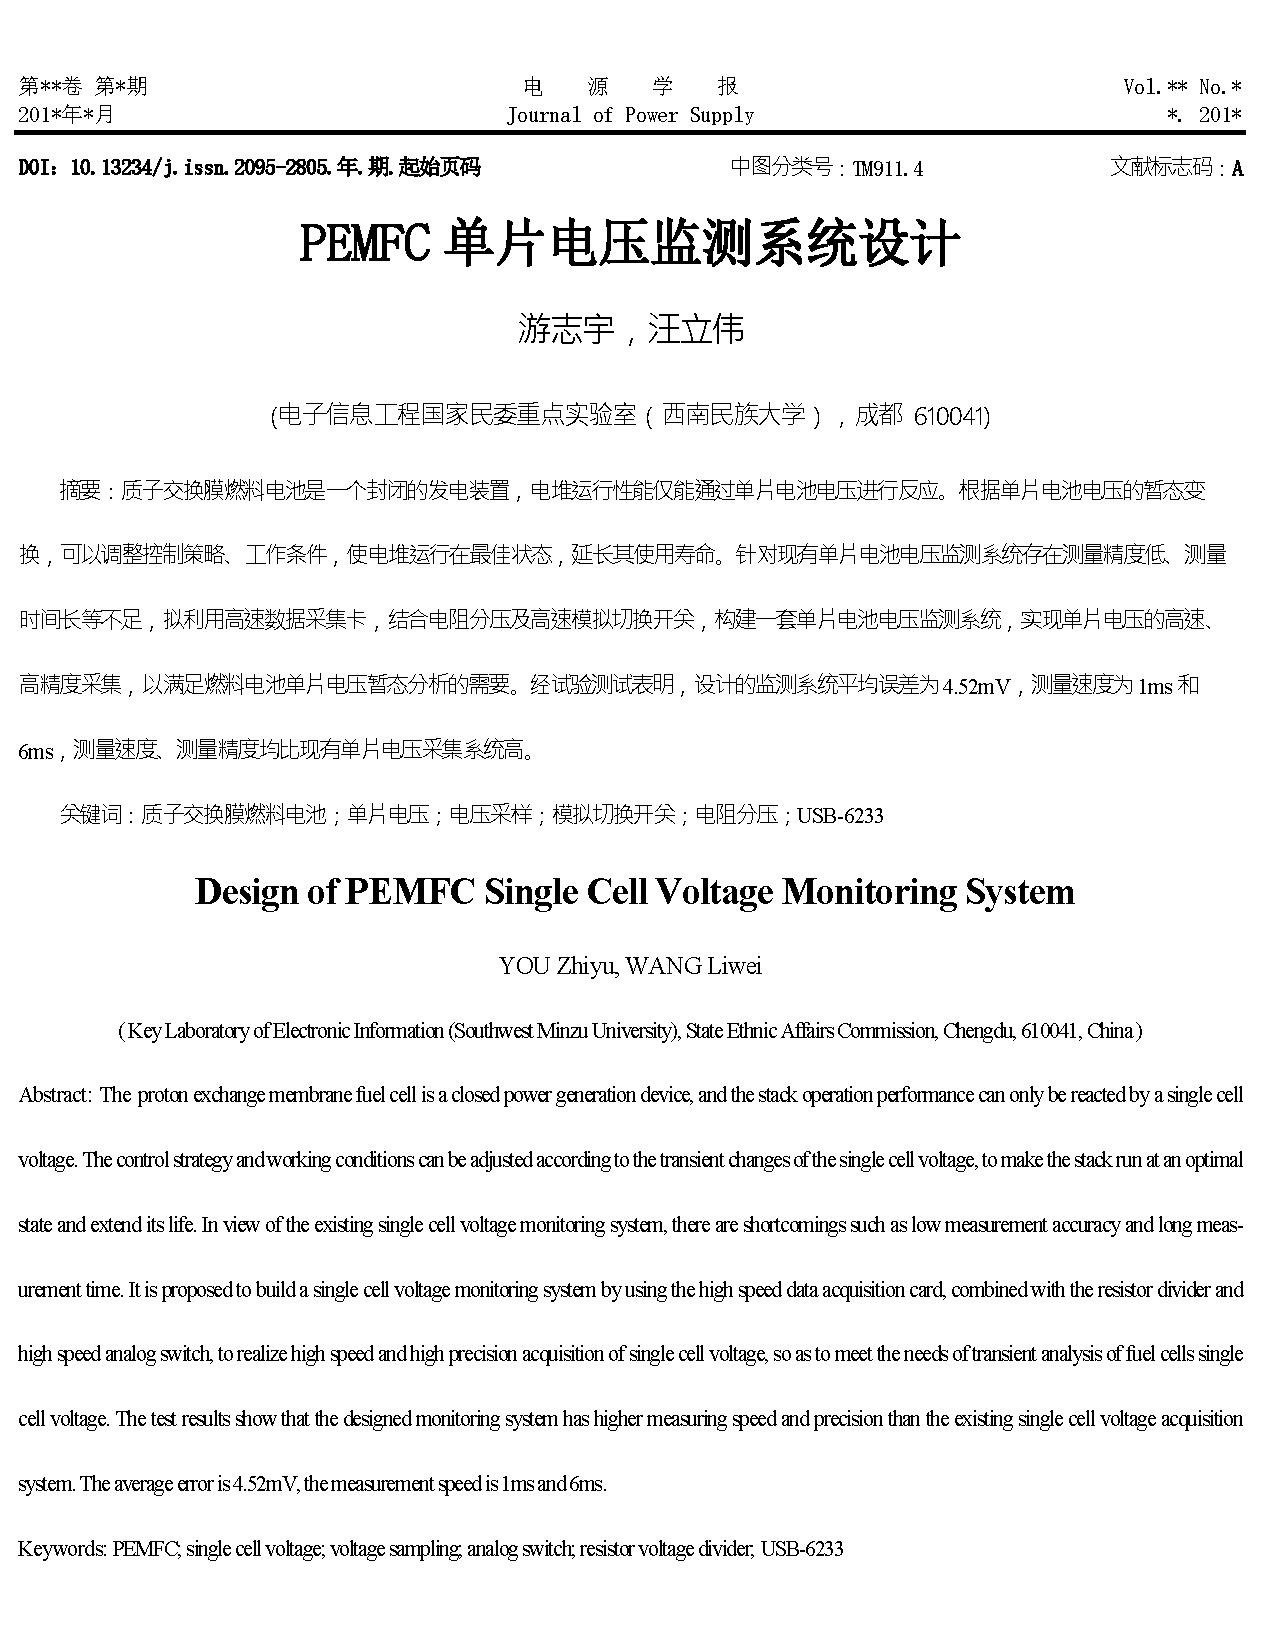
\includegraphics[scale=0.5, angle=0]{P1th.pdf}
\caption{Submission Paper1}
\label{fig:Submission Paper:PEMFC}
\end{figure}

\begin{itemize}
    \item Prepare and make a presentation about the two months work
\end{itemize}  
\par \vspace{-0.4cm}
\begin{figure}[h!]
\centering
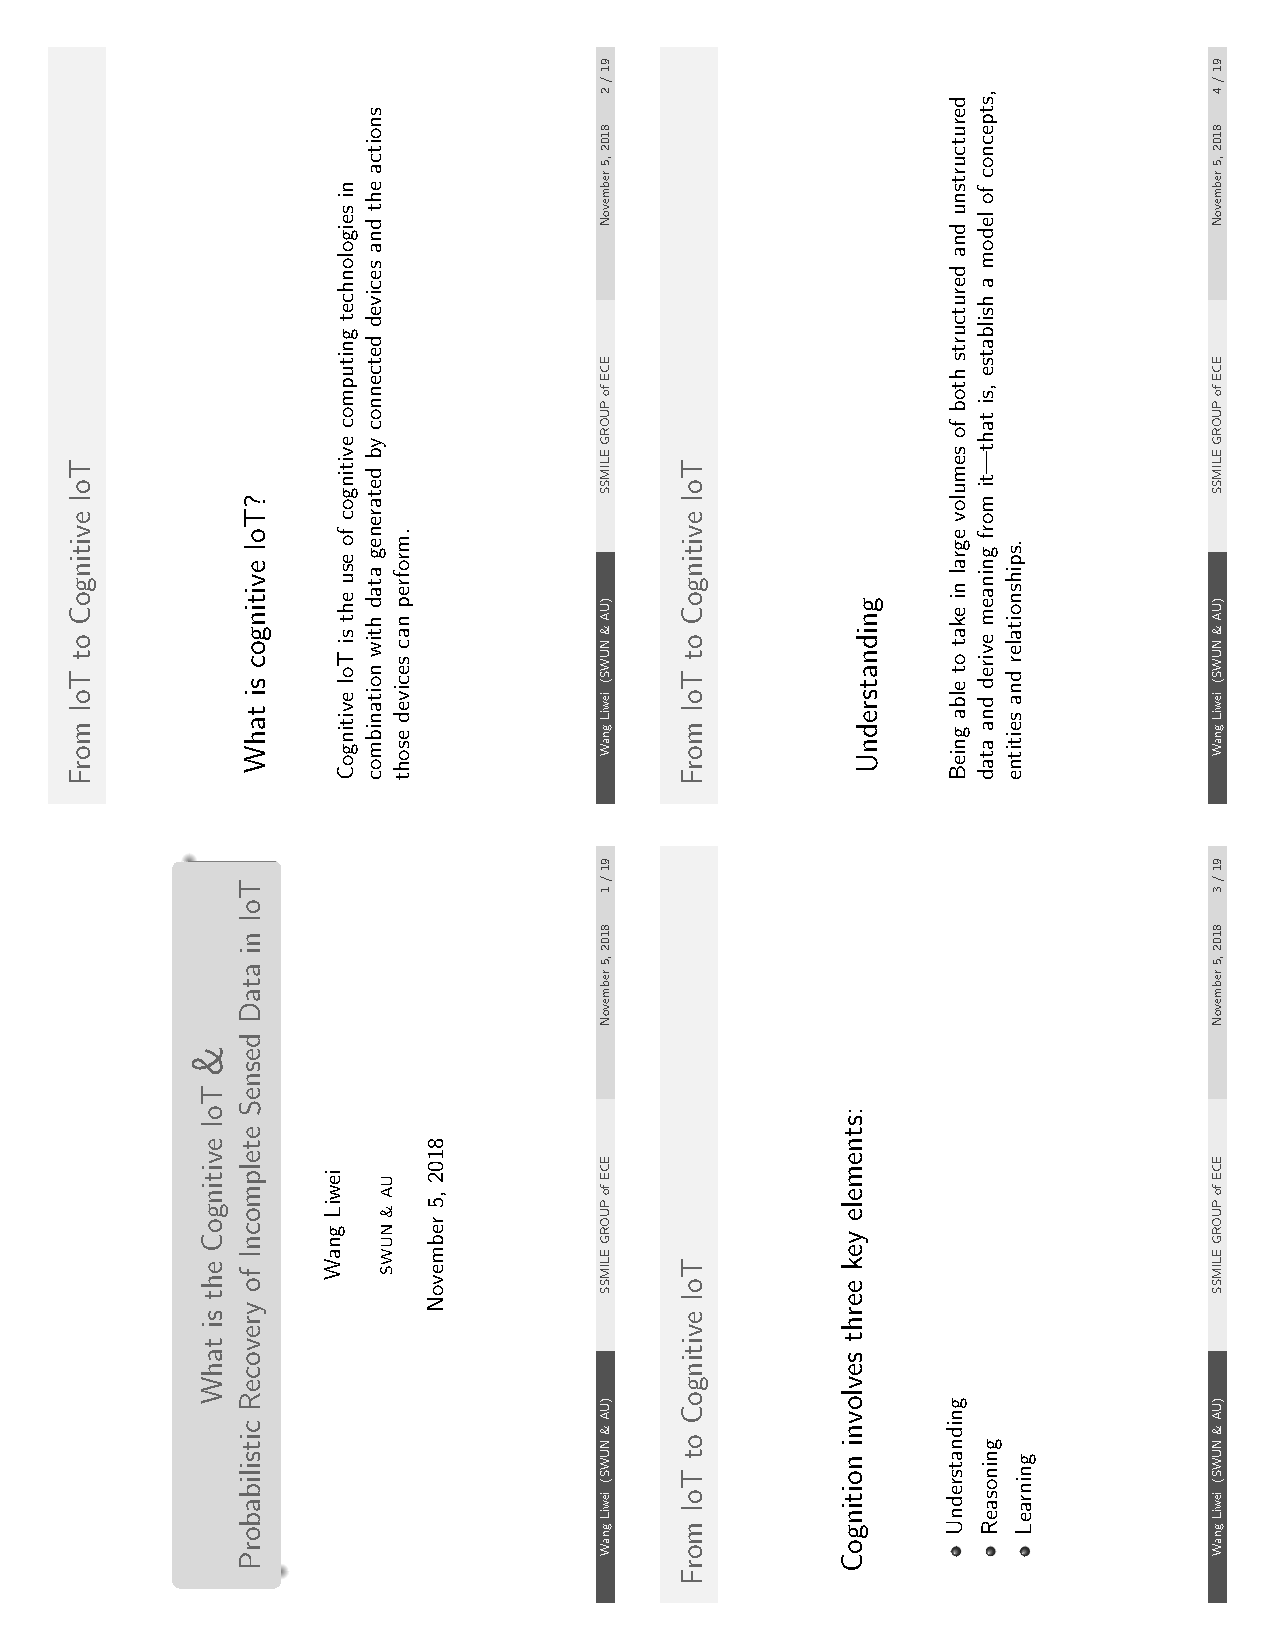
\includegraphics[scale=0.4, angle=-90]{Presentation_1_4.pdf}
\caption{My presentation}
\label{fig:My presentation}
\end{figure}


\begin{itemize}
    \item Participate in daily research work of the Team SSMILE.
\end{itemize}  
\par \vspace{-0.4cm}
In this month, there are also a weekly seminar and a weekly meeting with the supervisor. Prof.Zoran and PhD.Zhang make theirs presentation about the related research field.There are several academic conference was held  in the university. And the presentation of the PhD Thesis proposal was held too.I take part in all the academic activities.

\section*{\vspace{-1cm}}
All above is my reports about all I have been done within the past three month. It will be very grateful if the anyone kindly criticize and correct me.

\par
\vspace{1cm}
 \quad Best Regards

\vspace{2cm}
 \quad  \today


\vspace{1cm}
 \quad Comments of Supervisor:
\end{document}


% \citep{adams1995hitchhiker}
% \bibliographystyle{plain}
% \bibliography{references}